\clearpage
\section{Generalitati}


\bigskip

{\sffamily\color{black}
RODA va stoca toate informatiile in functie de dorinta celor care le pun in arhiva. Nivelele de acces la orice studiu se
vor stabili de catre proprietarii datelor. RODA este proiectata astfel incat sa ofere doua servicii:}

{\sffamily\color{black}
\ \ {}- serviciul de arhivare - asigurarea persistentei datelor in timp, indiferent de accidente, defectiuni hardware
sau software, modificari de tehnologie si orice alt fel de variabilitati ale mediului de lucru.}

{\sffamily\color{black}
\ \ {}- serviciul de publicare a datelor - care asigura celor interesati si indrituiti sa o faca posibilitatea
consultarii si obtinerii datelor din arhiva. }


\bigskip

{\sffamily\color{black}
Ambele servicii pot intalni probleme, iar infrastructura RODA este proiectata in asa fel incat sa permita depasirea
oricarei probleme sau situatie de forta majora. }


\bigskip

{\sffamily\color{black}
Arhivarea este considerata de RODA mai importanta decat publicarea - in cazul in care unul dintre servicii trebuie oprit
pentur a-l proteja pe celalalt, va fi oprita temporar publicarea pentru a proteja datele. Astfel de situatii pot
aparea, de exemplu, in cazul in care sistemul de publicare este tinta unui atac informatic care ar putea conduce la
expunerea datelor sau chiar la distrugerea lor. }


\bigskip

\section{Mentinerea integritatii datelor (arhivarea)}

\bigskip

{\sffamily\color{black}
Mentinerea integritatii datelor se refera la ansamblul de masuri luate pentru a evita pierderea lor, partiala sau
totala, indiferent de modul in care aceasta poate sa apara. }

{\sffamily\color{black}
Datele sunt urmatoarele:}

{\sffamily\color{black}
\ \ {}- Studiile sociologice, chestionarele, variabilele precum si toate informatiile atasate acestora (fisiere de date,
etc.), inclusiv informatii despre persoane si institutii implicate in realizarea acestora.}

{\sffamily\color{black}
\ \ {}- Datele cu privire la nivelele de acces la studii, drepturi, grupuri de acces, etc.}

{\sffamily\color{black}
\ \ {}- Datele de grupare a studiilor (cataloage, topicuri, etc).}

{\sffamily\color{black}
\ \ \ {}- Datele de acces la studii si jurnalele de modificare ale acestora}

{\sffamily\color{black}
\ \ {}- Programele software care asigura functionarea arhivei (aplicatii WEB, scripturi de automatizare, seturi de
configurare ale diverselor servicii)}

{\sffamily\color{black}
\ \ {}- Codul sursa.}


\bigskip

{\sffamily\color{black}
Riscurile de pierdere a datelor provin de obicei din urmatoarele accidente:}

{\sffamily\color{black}
{}- Disfunctionalitati ale infrastructurii hardware (hard-diskuri defecte, sisteme de date corupte de erori software,
manevrarea excesiva de catre utilizatori cu drepturi ridicate a functiilor de curatare). Principala protectie impotriva
acestui grup de probleme reprezinta redundanta datelor si backupul. Astfel, RODA va functiona conform schemei
urmatoare:}


\bigskip

{\sffamily\color{black}
\ \ Redundanta in timpul functionarii. Datele din primele doua categorii (studiile, \ informatiile conexe si nivelele de
acces) vor fi stocate in doua sisteme diferite: o baza de date SQL si un set de documente XML. Cele doua spatii de
stocare vor fi sincronizate intre ele dar altminteri independente. Aplicatia va putea reface oricare dintre spatiile de
stocare pe baza informatiilor din celalalt si aceasta se va putea face la nivelul unui singur studiu, grup de studii
sau la nivelul intregii baze de date.}

{\sffamily\color{black}
\ \ Backup on-line Infrastructura RODA contine un server de backup care va stoca o serie de copii zilnice ale datelor,
mergand in urma cu pana la 3 luni. Astfel, chiar daca accidenta se pot sterge anumite informatii, ele vor putea fi
recuperate din copiile de siguranta din zilele dinaintea stergerii. Serverul de backup nu va avea nici o legatura
functionala cu arhiva, va fi un agent extern care va citi datele si nici unul dintre utilizatorii obisnuiti RODA nu va
avea drept de acces pe el. Serverul de backup online va copia toate datele din lista de mai sus.}

{\sffamily\color{black}
\ \ Backup off-line. Periodic, datele RODA se vor scrie pe un dispozitiv de scriere pe banda magnetica. Benzile
magnetice vor contine toate datele necesare pentru recuperarea arhivei si vor fi stocate in alt loc, incuiate. Benzile
vor contine copii ale tuturor datelor din lista de mai sus }

{\sffamily\color{black}
Vor exista proceduri care vor acoperi toate scenariile posibile si care vor permite recuperarea datelor in toate
situatiile imaginabile.}


\bigskip

 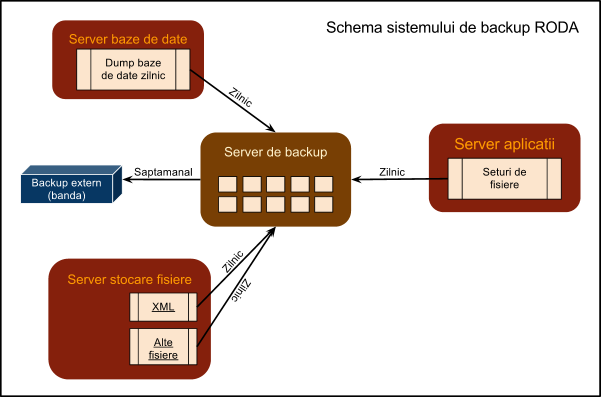
\includegraphics[width=6.2709in,height=4.1354in]{SecuritateaarhiveiRODA-img001.png} 


\bigskip

{\sffamily\color{black}
{}- Actiuni rauvoitoare ale utilizatorilor, administratorilor, persoanelor straine sau ale oricui altcuiva. }
\bigskip

\section{Securitatea aplicatiei si mediului de rulare}
\bigskip

{\sffamily\color{black}
Orice aplicatie WEB ruleaza intr-un mediu care contine o multitudine de programe externe, scrise si intretinute de alte
entitati, asupra carora RODA nu are si nu va avea niciodata control. Acestea includ, dar nu se limiteaza la: sisteme de
operare, biblioteci software specifice, servere software web, servere de baze de date, servere de e-mail si multe
altele. Toate aceste programe conlucreaza pentur asigurarea serviciilor RODA. Toate aceste programe pot avea (si de
multe ori au) vulnerabilitati care pot permite diverse atacuri, in special in cazurile in care instalarea si
administrarea lor nu se fac cu foarte multa atentie.}


\bigskip

{\sffamily\color{black}
Orice program ruleaza pe unul sau mai multe computere. Indiferent cat de sigur ar fi programul in ceea ce face el, orice
om care are acces fizic la computerul pe care ruleaza poate face ce doreste, daca are abilitatile necesare. De aceea, o
atentie speciala va fi acordata elementelor de securitate fizica (impiedicarea accesului la servere a persoanelor
neautorizate).}

\bigskip

\subsection{Securitatea mediului de rulare}
\label{securitatea_serverului}
\bigskip

\subsubsection{Securitatea fizica}

\bigskip

{\sffamily\color{black}
Securitatea fizica se refera la ansamblul de masuri luate pentru a impiedica persoanele neautorizate sa aiba acces
direct (fizic) la serverele pe care sunt stocate datele si aplicatiile RODA. Datorita modului in care a fost proiectat
sistemul, zona protejata este compusa doar din serverele pe care sunt instalate datele si aplicatiile arhivei, nici un
alt computer (statii de lucru, computere portabile) sau alte dispozitive (tablete, telefoane) nu vor stoca pe ele parti
din arhiva. }


\bigskip

{\sffamily\color{black}
Toate serverele pe care vor rula serviciile arhivei RODA vor fi montate intr-un dulap tehnic special, care va fi
incuiat. }


\bigskip

{\sffamily\color{black}
Dulapul tehnic se va afla intr-o camera tehnica. Accesul la aceasta camera tehnica se va face pe baza de cartela de
acces nominala si va fi inregistrat. }


\bigskip

{\sffamily\color{black}
Camera tehnica va fi supravegheata de un sistem de inregistrare video. }


\bigskip


\bigskip

\subsubsection{Securitatea logica}

{\sffamily\color{black}
Securitatea logica se refera la ansamblul de masuri luate pentru a impiedica o persoana neautorizata sa obtina acces
si/sau privilegii crescute pe serverele aplicatiei RODA pe cale electronica (prin retea). }


\bigskip

{\sffamily\color{black}
Protectia impotriva accesului neautorizat se face prin:}


\bigskip

{\sffamily\color{black}
\ \ {}- arhitectura serverelor}

{\sffamily\color{black}
\ \ {}- configurarea serviciilor pe servere, inclusiv servicii de monitorizare si interventie }

{\sffamily\color{black}
\ \ {}- reguli specifice de acces pentru administratori}


\bigskip

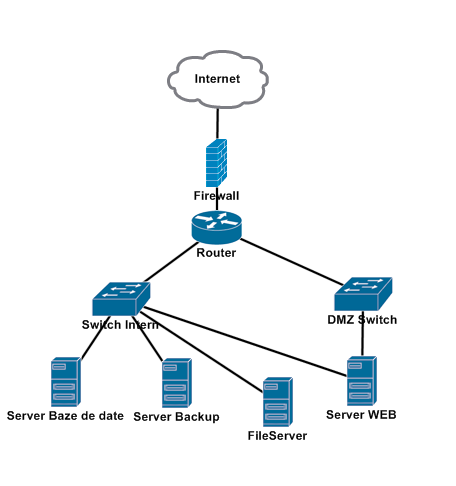
\includegraphics[width=4.75in,height=5.0626in]{SecuritateaarhiveiRODA-img002.png}

{\sffamily\color{black}
Arhitectura retelei este construita astfel incat intregul ansamblu de servere se este conectat la internet prin
intermediul unui router care va contine un firewall. Routerul este un computer care nu are nevoie de servicii
suplimentare, care nu are nevoie de utilizatori de sistem, un computer extrem de putin vulnerabil la exploatarea
erorilor software. Serverele sunt pozitionate in doua retele separate, una (DMZ) care are acces la internet si una
interna care este izolata.}

{\sffamily\color{black}
In aceasta configuratie serverele care contin informatia propriu-zisa, precum si serverul de backup nu pot fi accesate
direct din internet si, ca atare, nu vor putea fi tinta atacurilor informatice iar eventualele vulnerabilitati
nepublicate din programele care ruleaza pe ele nu vor putea fi atacate fara compromiterea routerului (extrem de
dificila).}


\bigskip

{\sffamily\color{black}
Configurarea serviciilor pe servere este facuta conform urmatoarelor principii:}

{\sffamily\color{black}
\ \ {}- fiecare server are disponibile doar serviciile strict necesare}

{\sffamily\color{black}
\ \ {}- fiecare serviciu dintre cele strict necesare nu are incarcate decat componentele care de care este nevoie pentru
a functiona arhiva.}

{\sffamily\color{black}
\ \ {}- numarul utilizatorii (atat cei umani cat si cei de sistem) este cel minim necesar}

{\sffamily\color{black}
\ \ {}- serviciile cu acces din exterior sunt monitorizate de sisteme care blocheaza accesul adreselor IP de pe care se
incearca mai mult de 5 autentificari nereusite}

{\sffamily\color{black}
\ \ {}- serviciile care implica transfer regulat de date intre servere sunt conectate la canale criptate.}

{\sffamily\color{black}
\ \ {}- partitiile care contin fisiere temporare, cu drept de scriere pentru orice aplicatie sunt incarcate de catre
sistemul de operare fara permisiunea de executie a aplicatiilor. }

{\sffamily\color{black}
\ \ {}- jurnalele de sistem sunt replicate pe serverul de backup}

{\sffamily\color{black}
\ \ {}- Intreaga retea este monitorizata automat de un serviciu specializat, cu agenti pe fiecare dintre servere care
poate alerta administratorul de sistem in cazurile in care apar exceptii de la comportamentul normal al acestora. }


\bigskip

{\sffamily\color{black}
RODA va utilizeaza exclusiv programe open-source. Acestea sunt mai usor de monitorizat din punct de vedere al
vulnerabilitatilor, reparatiile acestora apar mai repede si pot fi aplicate de catre administratorii serverului in
cazuri extreme. Administratorul de sistem va urmari listele de discutii, va efectua toate update-urile de software
necesare si va efectua teste periodice care sa acopere principalele vulnerabilitati ale fiecarui program in parte. }


\bigskip

{\sffamily\color{black}
Administratorii serverelor pot accesa reteaua doar prin canale criptate si nu se pot autentifica direct ca utilizatori
cu drepturi ridicate. }

\subsection{Securitatea WEB}


\bigskip

{\sffamily\color{black}
Majoritatea operatiilor cu date ale arhivei RODA, si TOATE operatiile care implica alte persoane decat administratorii
bazei de date se vor face prin intermediul unei interfete WEB. Datorita modului de rulare si protocoalelor implicate,
majoritatea interfetelor WEB pot fi afectate de o vulnerabilitati similare. In cele ce urmeaza, vom detalia modul prin
care designul arhivei RODA va evita cele mai importante astfel de vulnerabilitati. Lista acestora urmeaza clasificarea
OWASP (Open Web Application Security Project -
\href{https://www.owasp.org/}{\textcolor[rgb]{0.06666667,0.33333334,0.8}{https}}\href{https://www.owasp.org/}{\textcolor[rgb]{0.06666667,0.33333334,0.8}{://}}\href{https://www.owasp.org/}{\textcolor[rgb]{0.06666667,0.33333334,0.8}{www}}\href{https://www.owasp.org/}{\textcolor[rgb]{0.06666667,0.33333334,0.8}{.}}\href{https://www.owasp.org/}{\textcolor[rgb]{0.06666667,0.33333334,0.8}{owasp}}\href{https://www.owasp.org/}{\textcolor[rgb]{0.06666667,0.33333334,0.8}{.}}\href{https://www.owasp.org/}{\textcolor[rgb]{0.06666667,0.33333334,0.8}{org}}).
OWASP publica in fiecare an o lista cu cele mai importante vulnerabilitati ale aplicatiilor WEB. }


\bigskip

\subsubsection{Injectare (SQL, LDAP, OS) }


\bigskip

{\sffamily\color{black}
Injectarea este procedura de atac prin care se introduce intr-un formular care urmeaza a fi trimis la server o
succesiune de comenzi cu scopul de a determina serverul sa le execute. Injectarea este considerata ca fiind cel mai
important risc de securitate a unei aplicatii WEB, estimandu-se ca o aplicatie cu trafic normal poate primi pana la 70
de incercari de injectare pe ora. Cea mai frecventa modalitate de atac prin injectare este injectarea SQL. Aceasta
afecteaza aplicatiile care nu filtreaza datele care sunt trimise bazei de date in formularele disponibile
utilizatorilor. }


\bigskip


\bigskip


\bigskip


\bigskip

 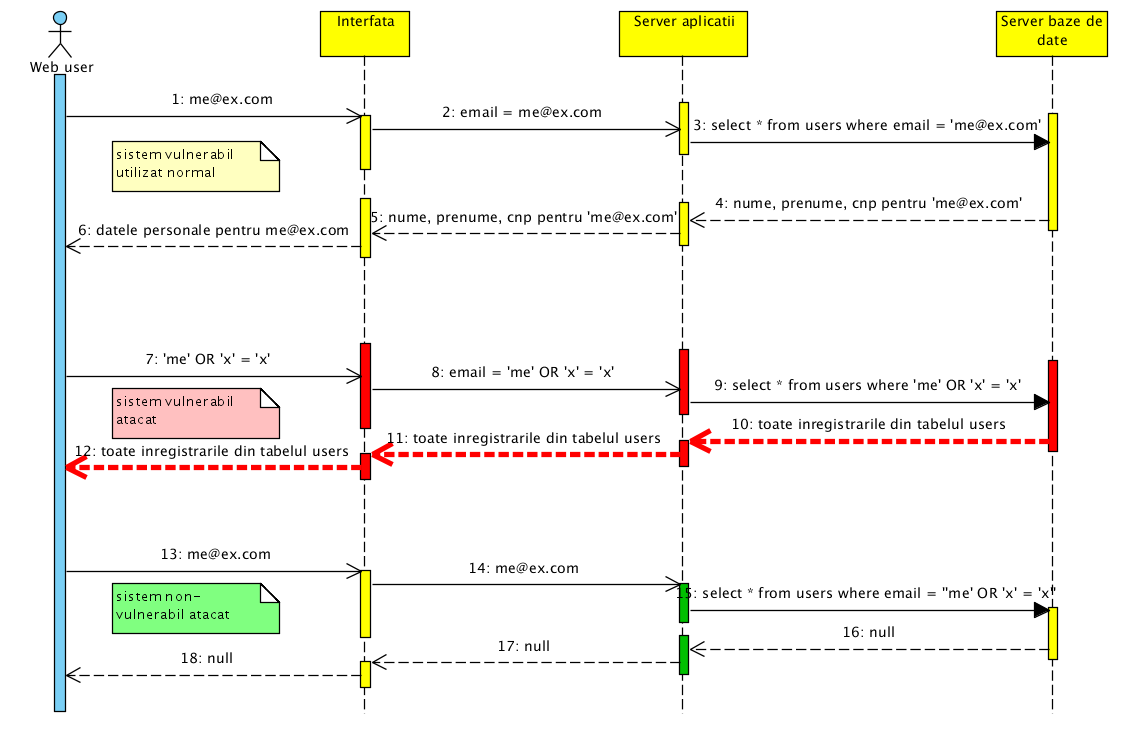
\includegraphics[width=7.1146in,height=4.6146in]{SecuritateaarhiveiRODA-img003.png} 


\bigskip

{\sffamily\color{black}
Moduri de evitare a injectiei SQL. Evitarea injectiei SQL se face in RODA in mai multe etape:}
\begin{enumerate}
  \item 
Control strict al proprietatilor datelor introduse si validarea exacta a caracteristicilor datelor. De exemplu,
daca intr-un formular un utilizator va trebui sa introduca o adresa de e-mail, aplicatia va verifica sirul de caractere
introdus si nu ii va permite sa treaca mai departe daca acesta nu respecta regulile stricte de forma a unei adrese de
email. Daca utilizatorul trebuie sa introduca un numar de telefon, de asemenea. Se vor verifica si valida tipurile de
date, lungimea (numarul de caractere) ale acestora, precum si prezenta.
\item
Proiectarea aplicatiei astfel incat nici o funtionalitate a acesteia
sa nu ocoleasca modelul, componentul responsabil de comunicarea cu baza de date.
\item
Controlul strict al datelor si proprietatilor acestora la nivelul
modelului, adica a codului responsabil de comunicarea directa cu baza de date. Astfel, din punct de vedere al functiilor modelului, orice data care va intra in
baza de date este suspecta si trebuie validata, chiar daca aceasta vine pe canale considerate sigure.
\item
Utilizarea interogarilor duale pentru introducerea de date in baza
de date. Exista doua moduri de a introduce date intr-un tabel prin intermediul limbajului SQL:
\begin{description}
	\item [direct;] de ex.: INSERT INTO LANGUAGE (ID, NUME) VALUES (1,
`ROMANA')
	\item [prin preparare si executie.] Metoda presupune prepararea interogarii folosind
semne de intrebare in locul valorilor si executia parametrizata a interogarii: 
PREPARE: INSERT INTO LANGUAGE (ID, NUME) VALUES (?, `?') 
urmata de
EXECUTE: (1, `ROMANA'). 
Executia parametrizata a interogarilor asigura faptul ca orice fragment de date va intra exact
acolo unde ii e locul in baza de date si nimeni nu va putea, printr-o combinatie a interogarii aplicatiei si a datelor
introduse sa determine serverul sa execute altceva. 
\end{description}
Toate interogarile modelului RODA sunt executate prin metoda duala. Modelul este conceput astfel incat absolut toate
interogarile, chiar daca nu par a fi periculoase la prima vedere, sa fie trimise catre serverul de baze de date in mod
parametrizat.
\end{enumerate}

\bigskip

\subsubsection{Exploatarea deficientelor de autentificare si management al
sesiunii}

\bigskip

{\sffamily\color{black}
Deficientele de autentificare si de management al sesiunii conduc la executia de operatii neautorizate. Exista mai multe
metode prin care se poate ajunge aici, toate presupunand ca un utilizator reuseste cumva sa obtina un cod (sesiune,
cookie, parola) apartinand altui utilizator. Este aproape imposibila o protectie totala impotriva acestui tip de atac
(cineva poate pur si simplu sa spuna altcuiva propria parola) dar, de regula, se incearca sa se evite obtinerea
accesului fara voia celui care il are. Pentru aceasta, se vor lua urmatoarele masuri:}
\begin{itemize}
\item
informatiile tipice sesiunii utilizatorului vor fi stocate in baza de date
\item
sesiunea de lucru va expira la un timp scurt de la ultima actiune, iar programul responsabil pentru expirarea sesiunii
nu va avea nici o legatura cu aplicatia web
\item 
sistemul va impune automat un standard ridicat al parolelor utilizate de
catre utilizatori
\item 
sistemul va bloca accesul adreselor ip care acumuleaza prea multe incercari esuate de autentificare
\item
toate procedurile de autentificare si operatii cu datele de autentificare
se for face prin comunicare criptata (https) pentru a evita interceptarea datelor de catre altcineva.
\item 
modificarea codului de sesiune la fiecare solicitare, cu pastrarea datelor, pentru a evita atacuri de tip ``fixare de
sesiune''
\item
refuzul id-urilor de sesiune care nu sunt generate de RODA
\item
utilizarea argumentului \textit{HttpOnly}\textit{ }pentru cookie-urile
trimise de aplicatie.
\end{itemize}

\subsubsection{XSS (Cross Site Scripting)}

\bigskip

{\sffamily\color{black}
Cross Site Scripting presupune introducerea in continutul arhivei a unor fragmente de cod care, executate in programele
de navigare a utilizatorilor, pot determina o multime de comportamente distructive, in special pe computerele care
viziteaza site-ul. Fragmentele de cod pot fi introduse in principal in doua categorii de informatie stocata pe server:
informatia aflata in baza de date si fisierele statice care folosesc la constructia interfetelor dinamice (ex:
javascript). Astfel, protectia impotriva acestui tip de atacuri trebuie sa fie duala: protectia datelor introduse in
baza de date si protectia fisierelor statice. }


\bigskip

 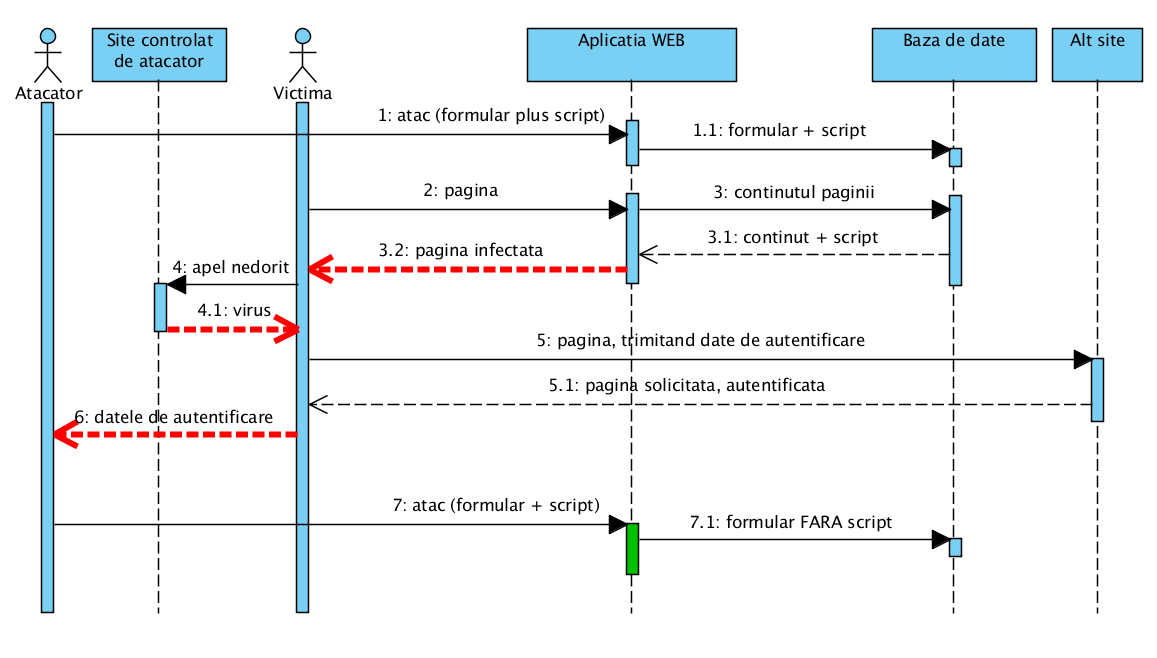
\includegraphics[width=6.7602in,height=3.8437in]{SecuritateaarhiveiRODA-img004.png} 


\bigskip

{\sffamily\color{black}
Protectia bazei de date: }

\bigskip

{\sffamily\color{black}
Scripturile XSS pot ajunge in baza de date prin formularele comune puse la dispozitie utilizatorilor pentru introducerea
datelor. Pentru a preveni acest lucru, toate datele introduse in baza de date vor fi atent filtrate, conform
urmatoarelor reguli:}

{\sffamily\color{black}
\ \ {}- nu se va permite introducerea in baza de date a nici unui cod javascript sau alt fel de cod care poate fi
executat in navigatorul client. }

{\sffamily\color{black}
\ \ {}- nu se va permite introducerea in baza de date a nici unei instructiuni de tip IFRAME, care permite atragerea
continutului de pe site-uri externe. }

{\sffamily\color{black}
\ \ {}- interfata pentru utilizatori altii decat administratorii RODA nu va putea introduce in baza de date decat un
subset limitat al limbajului HTML, cu scop de formatare. }


\bigskip

{\sffamily\color{black}
Protectia fisierelor statice}
\begin{itemize}
  \item 
  Fisierele statice (javascript, css) vor fi stocate read-only.
  \item 
  Fisierele statice se vor servi prin intermediul unui asset manager care va stoca o amprenta a fiecaruia. In cazul in
care apar modificari despre care sistemul nu ``stie'' servirea acestora va fi oprita.
\end{itemize}

\bigskip

\subsubsection{Referinte directe catre obiectele interne}

\bigskip

{\sffamily\color{black}
Referintele directe catre obiecte interne se refera la modul in care sunt construite URL-urile unei aplicatii web, in
special, la faptul ca acestea nu trebuie sa permita vizitatorilor sa ``ghiceasca'' detalii de implementare din spatele
interfetei. Aceasta nu este o problema in sine daca nu este cuplata cu o schema de autentificare care nu verifica
fiecare solicitare. }


\bigskip

{\sffamily\color{black}
Prin modul in care este proiectat, sistemul de autentificare al RODA va verifica drepturile utilizatorilor la fiecare
pas al acestora, iar obiectele importante (studii, cataloage) vor fi obiectul unui sistem de acl-uri care se va asigura
ca un utilizator nu poate accesa un anumit studiu chiar daca poate sa-i ghiceasca adresa. De asemenea, prin utilizarea
unul sistem de tip Model View Controller, adresele obiectelor nu vor fi mapari directe ale tabelelor bazei de date. }


\bigskip

\subsubsection{Slaba configurare a serverului pe care ruleaza aplicatia. }


\bigskip

{\sffamily\color{black}
Securitatea serverului a fost discutata in capitolul
\ref{securitatea_serverului}.}


\bigskip

\subsubsection{Expunerea datelor sensibile}


\bigskip

{\sffamily\color{black}
Problemele legate de expunerea datelor sensibile sunt in general determinate de insuficienta protectie a numerelor de
carduri de credit, date de identificare (ex: cnp) sau a datelor de autentificare. RODA nu va stoca date financiare,
nici carti de credit, iar datele personale ale utilizatorilor sistemului vor fi disponibile numai in cazuri speciale.
Parolele tuturor utilizatorilor arhivei nu vor putea fi cunoscute de nimeni, pentru ca vor fi stocate direct criptate
in baza de date, comparatia necesara pentru autentificare facandu-se prin criptarea similara a parolei oferite in
momentul intrarii in sistem. Parolele utilizatorilor nu vor exista nicaieri altfel decat criptate.}


\bigskip

{\sffamily\color{black}
De asemenea, RODA va incerca sa nu solicite utilizatorilor sai mai multe date decat sunt absolut necesare pentru
operarea arhivei la nivelul la care se afla fiecare utilizator. Toate operatiile in care utilizatorii vor trebui sa
transmita date personale (parole) catre aplicatia RODA vor fi facute prin canale criptate. }

\bigskip

\subsubsection{Lipsa controlului de acces la nivelul functiilor serverului}

\bigskip

{\sffamily\color{black}
Aceasta vulnerabilitate este oarecum asemanatoare cu cea de la punctul 4 si se refera la accesarea de catre utilizatori
a unor optiuni pentru care nu au drepturi de executie, fie prin aparitia lor eronata in meniuri, fie prin incercari
succesive de a descoperi noi functionalitati. }

\bigskip

{\sffamily\color{black}
Sistemele de navigatie (meniuri, linkuri) din interiorul aplicatiei RODA vor fi generate de un modul care va tine seama
de drepturile de acces, astfel, nici un utilizator nu va avea disponibile optiuni pe care nu are dreptul sa le
acceseze. }

\bigskip

{\sffamily\color{black}
Prin modul de proiectare al aplicatiei RODA, autentificarea se verifica la fiecare actiune a utilizatorului, astfel,
chiar in situatia in care acesta poate ``ghici'' un anumit url de apel al unei functii pe care nu o vede in interfata,
serverul va refuza executia acesteia daca utilizatorul nu are drepturile necesare.}

\bigskip

\subsubsection{CSRF (Cross Site Request Forgery)}

\bigskip

{\sffamily\color{black}
Falsificarea solicitarii HTTP - este situatia in care un anumit component al aplicatiei este accesat direct din alt
site. Aceasta conduce catre trimiterea unor modificari catre sistem, fara sa se utilizeze pagina cu formularul conceput
pentru aceasta, si, in functie de proiectarea sistemului, ocolindu-se procedurile de validare daca acestea sunt
prezente doar in formular sau intreg sistemul de autentificare.}

\bigskip

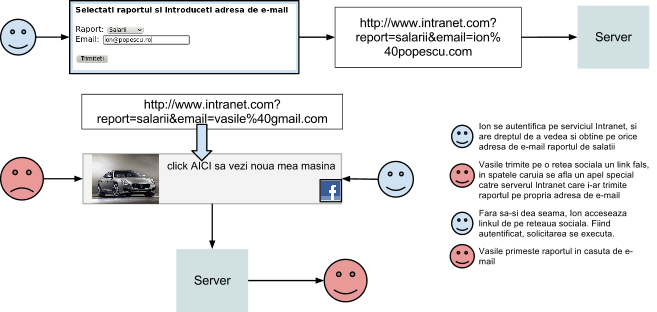
\includegraphics[width=6.8437in,height=3.6457in]{SecuritateaarhiveiRODA-img005.png} 

\bigskip

{\sffamily\color{black}
Pentru evitarea acesui gen de atac, aplicatia RODA va lua urmatoarele masuri:}

{\sffamily\color{black}
\ \ {}- toate formularele care conduc catre inserarea de noi date sau modificarea datelor existente for folosi o
amprenta speciala (token) pe care serverul o va genera odata cu formularul si o va verifica la primirea datelor.
Astfel, daca datele nu au provenit din formular, continand astfel si amprenta respectiva, serverul va refuza sa opereze
modificarile. Amprenta va expira dupa un timp destul de scurt, astfel incat sa se evite posibilitatea ghicirii
acesteia. }

{\sffamily\color{black}
\ \ {}- toate URL-urile aplicatiei vor fi verificate strict astfel incat sa aiba
numarul corect de parametri si pozitionarea corecta}

{\sffamily\color{black}
\ \ {}- nici un apel de tip GET nu va putea sa faca modificari in baza de date sau in orice alt strat de stocare
persistenta a datelor. }


\bigskip

\subsubsection{Utilizarea componentelor cu vulnerabilitati cunoscute}

\bigskip

{\sffamily\color{black}
Evitarea vulnerabilitatilor compoenntelor externe se face prin urmatoarele operatiuni care vor fi realizate ori de cate
ori va fi nevoie:}

{\sffamily\color{black}
\ \ {}- Mentinerea la zi a tuturor componentelor software, aplicarea tuturor update-urilor publicate de producatorul
sistemului de operare}

{\sffamily\color{black}
\ \ {}- Monitorizarea site-urilor sistemului de operare, ale producatorilor componentelor software, listelor de discutii
si altor sisteme de comunicare a vulnerabilitatilor descoperite si repararea, inlocuirea sau inchiderea serviciilor sau
componentelor care pot fi atacate. }


\bigskip

\subsubsection{Redirectari nevalidate }

\bigskip

{\sffamily\color{black}
Se refera la site-uri care folosesc redirectarea pentru a oferi acces la alte resurse, fara validarea solicitarii care a
condus la necesitatea redirectarii. RODA va verifica autentificarea si autorizarea la fiecare solicitare a
utilizatorilor astfel incat orice apel, chiar daca acesta ar putea duce la o redirectare va trece prin filtrul
verificarilor autenticitatii utilizatorului. }
